

\section{Introduction}
Efficiency in energy usage is a well-known topic. In the majority of fields, the purpose is to minimize the energy consumption of electrical devices and components. Modern times even see energy classification (A, B,... F) for homes, cars, and electronic products, to provide the consumer an indication of the energy consumption of their devices, which will reflect on their power bill. This criterion is extended even to the hardware components of a computer.
Figure~\ref{fig:soa_comparaisoncpu}\footnote{\url{https://www.cpubenchmark.net/compare/Intel-i9-12900KS-vs-Intel-i9-12900KF/4813vs4611}} presents a comparaison between to Intel CPU, the i9-12900KS and the i9-12900KF. The difference between these two CPUs is that the KS has an unlocked multiplier, allowing it to be overclocked. As a result, the basic consumption is less than the KF. This statistic also estimates the average power consumption of these two CPUs each day, as well as the monetary equivalent, to make people more aware of the values of energy consumption rather than the raw data.


\begin{figure}
    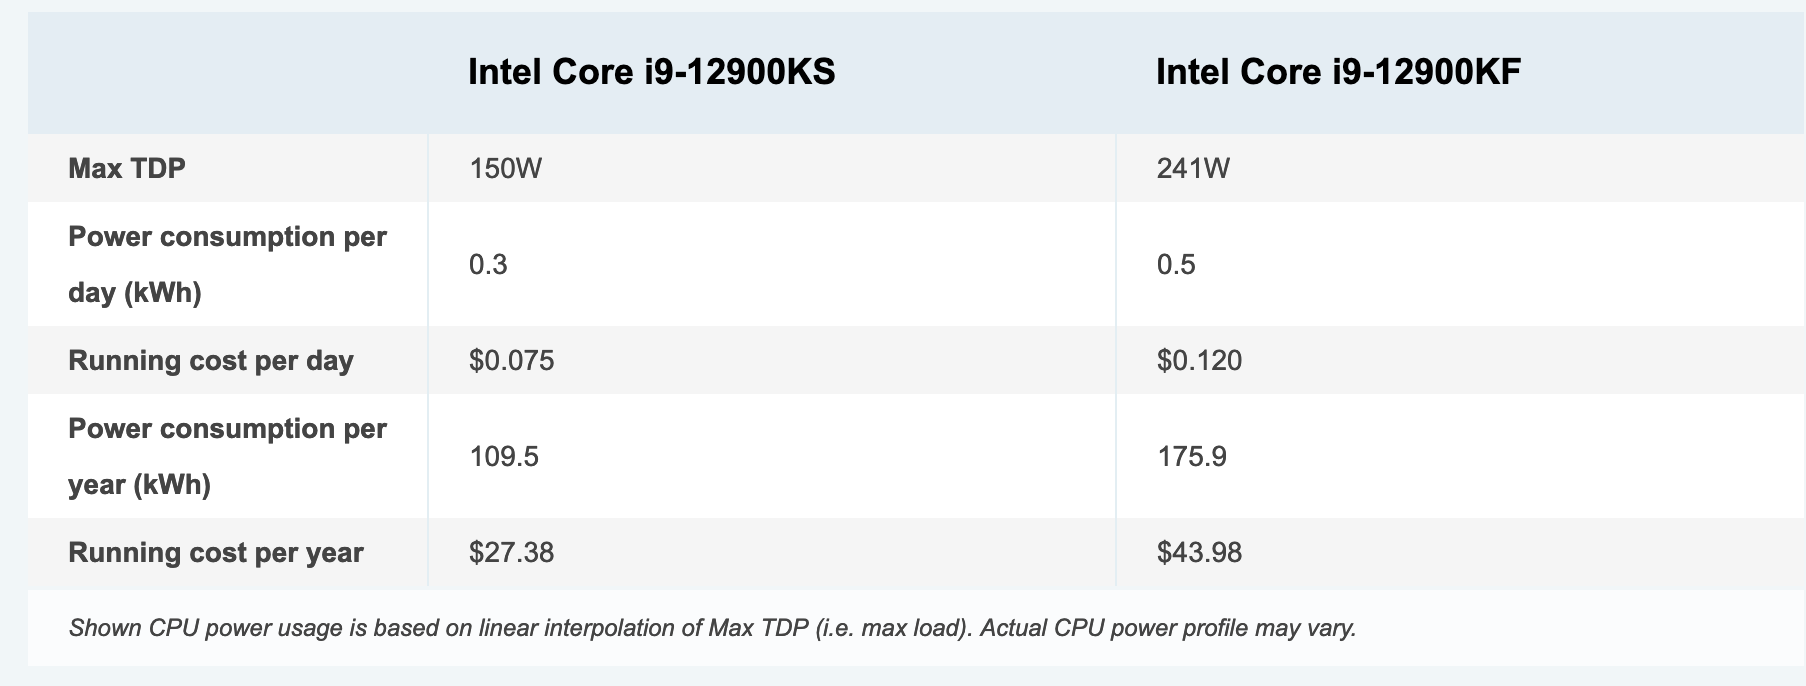
\includegraphics[width=\linewidth]{imgs/cpu_cost_comparaison}
    \caption{Electrical cost comparasion between two cpus }
    \label{fig:soa_comparaisoncpu}
\end{figure}

In computer science, the objective is essentially the same. Numerous studies have been conducted on energy optimization. Some of these studies concentrate on minimizing energy consumption at the hardware level, while others optimize energy consumption via software.

% displays the digital energy consumption distribution in 2017 \cite{andrae2015global}. ("p" for production and "u" for usage). 
% It demonstrates that both the production and consumption stages have substantial effects.
% In addition, the utilization expenses of data centers, networks, and terminals are also substantial (19 percent , 16 percent and 20 percent respectively).


As an example \citeauthor{avgerinou_trends_2017} evaluated the development of power use effectiveness (PUE) in data centers thkat belongs to various organizations participating in the European code of conduct for energy efficiency program \cite{avgerinou_trends_2017}.
The research found a gradual decline in the PUE of data centers, which measures the ratio of the overall energy supplied to the energy used by IT equipment.
A low PUE implies that the majority of energy is utilized to power the data center's IT equipment, while just a small amount is needed for cooling and lighting.

We will place a greater emphasis on the software level in order to decrease the amount of energy that is used, more particularly on the execution phase of the program cycle.
We will be proceeding through an empirical analysis of the energy consumption of the software while changing some components of the source code without impacting its behavior.
In order to do this, we will elaborate a benchmarking process and a set of tools that are intended to assist practitioners in better comprehending and optimizing the energy usage of their applications.
Thus, we will begin by examining the state of the art of empirical analysis and retrieving the best empirical experimentation methodologies in the research field. Then, we will narrow these practices down to computer science so that we can finally adapt them to energy consumption.

Section~\ref{sec:soa_benchmarking} will discuss the pitfalls and best practices associated with empirical research before applying them to our field of interest.
After that Section~\ref{sec:soa_energymeasurement} describes software energy measurements.
It provides examples of hardware and software measuring instruments and describes their differences, benefits, and drawbacks. It also examines the sources of energy measurement variations, which represent a significant obstacle to achieving precise readings and a higher accuracy.
Then, in section \ref{section:soa_energyoptimization}, we will go through some of the previous work on improving the energy consumption of softwares.

\newpage
\section{Benchmarking}\label{sec:soa_benchmarking}
This section will go through the flaws and best practices of empirical research before applying them to our topic of study.

\subsection{Threats \& Challenges}
A successful benchmark must meet three criteria.
First, it must be \textbf{reproducible} in order for others to imitate it.
Second, the findings should be \textbf{accurate},which implies that we should expect the same results each time we run the benchmark.
Finally, it should \textbf{represent} reality.
In other words, the experiment's findings should be applicable outside of the research lab as well.
The aim of \textbf{representativeness} in this thesis is the manufacturing environment.
As a result, the experiments should reflect what happens in production contexts.

\subsubsection{Reproducibility}\label{subsec:soa_reproducibility}

Experiment reproducibility is frequently listed as one of the most difficult challenges faced by researchers. Reproducing an experiment has been one of the major tools science has used to help establish the validity and importance of scientific findings since the Philosophical Transactions of the Royal Society were established in 1665~\cite{hankins1986debate}. In point of fact, many of the outcomes are not duplicable,\footnote{Trouble at the lab, The Economist, 19 October 2013;  www.economist.com/news/briefing/ 21588057-scientists-think-science-self-correcting- alarming-degree-it-not-trouble.} which led to a \emph{replication crisis}.
As a result of the crisis affecting the majority of empirical studies, most reviews now include reproducibility as a minimum standard for judging scientific merit~\cite{peng2011reproducible}.
One of the criteria for  supporting reproducibility is the publication of the dataset and the algorithms run on the raw data to derive the results.
There is even some disagreement about what the terms "reproducibility" or "replicability" by themselves mean \cite{goodman2016does}.
According to \cite{echtler2018open}, \emph{replicability} extends \emph{reproducibility} with the ability to collect a new raw dataset comparable to the original one by re-executing the experiment under similar conditions, instead of just the ability to get the same results by running the statistical analyses on the original data set.


\subsubsection{Accuracy}
According to Oxford, \emph{accuracy} means \href{https://www.lexico.com/definition/accuracy}{"technical The degree to which the result of a measurement, calculation, or specification conforms to the correct value or a standard"}.
In our case, this means the ability to run the benchmark multiple times with low variation. This can be achieved by controlling the experiment environment, allowing less room for random factors.
In biology, chimestry, and electronics, they use clean rooms, which are environments where pollutants like dust, airborne microbes, and aerosol particles are filtered out and factors like humidity, air flow, and temperature can be regulated. As for empirical analysis, the accuracy can be measured by numeric metrics such as the variance, the standard deviation (STD), and the interval inter quartile (IRQ).
Section~\ref{sec:energy_variation} will go over the accuracy in the subject of energy optimisation.

\subsubsection{Representativeness}
As obvious as it seems, the reason for executing benchmarks is to validate ideas so we can use them in real life.
However, this means that those benchmarks have to represent reality somehow. In Social sciences, this can be achieved by selecting a representative sample size. \citeauthor{omair2014sample}~\cite{omair2014sample} presents a guideline on to achieve a such representativeness.
As for computer science. The field of benchmarking is still in its infancy, and there is no consensus on how to achieve representativeness. Howerver many attemps have been made to provide a set of benchmarks for specific purpose.
For example, the \href{https://www.spec.org/}{Standard Performance Evaluation Corporation} (SPEC) provides a set of benchmarks for CPU performance evaluation. This sets covers a wide range of use cases such as  CPU17 for testing the CPU \footnote{\url{https://www.spec.org/cpu2017/}}, SPECviewperf\footnote{\url{https://gwpg.spec.org/benchmarks/benchmark/specviewperf-2020-v3-1/}} for Graphic usage and
one can cite stressNg when it comes to benchmark the hardware compoment, the SPEC benchmark when it comes to benchmark the software performance,and SPECPower\footnote{\url{https://www.spec.org/power_ssj2008} }.
NASA Parallel Benchmarks (NPB~\footnote{\url{https://www.nas.nasa.gov/publications/npb.html}} )
and HPCchallenge \footnote{\url{https://www.hpcchallenge.org/}} are two other examples of benchmarking sets that are created to represent the high performance computing.
As for programming languages we can cite Computer Language Benchmarks Game~\footnote{\url{https://benchmarksgame-team.pages.debian.net/benchmarksgame/index.html}}, which is a collection of benchmarks for various programming languages. The benchmarks are designed to be small, self-contained, and easy to implement in any language. The benchmarks are also made in a way to represent of most of the typical real-world workloads in an isolated manner.
Dacapo~\cite{blackburn2006dacapo} and renaissance~\cite{renaissance} are another example of a benchmarking set that are created to represent the Java Virtual Machine (JVM) performance.
On the other hand, a new sort of test has arisen within the software development life cycle. This type is known as stress testing, and it is used to assess the software's robustness and reliability before releasing it to the public. gatling~\footnote{\url{https://gatling.io}} and TCPCopy\footnote{\url{https://github.com/session-replay-tools/tcpcopy}} are great  examples of a stress testing tools that are used to test the performance server applications.

% But, how can we assure that the benchmark is representative? honestly i don't know. and we can't generalize this. but there are some works that have been done for this.
% Basically, when we aim to benchmark something, we create a mockup version of the situation in which we want it to work.
% First, we can talk about the benchmarking and their selection, then we will talk about the stress benchmark for some applications, and finally we will bring this representativeness in our case and how can we get closer to the energy consumption behavior of a software between the benchmark environnement and the production one.
% Recently, the research community has been investigating typical "crimes" in systems benchmarking and established guidelines for conducting robust and reproducible evaluations~\cite{DBLP:journals/corr/abs-1801-02381}.

% We first start by defining the word \textbf{benchmark},  
% definition :benchmark: [noun] something that serves as a standard by which others may be measured or judged.
% that serves as a basis for evaluation or comparison (as of computer system performance)
\subsubsection{Impact of these Challenges in the Empirical Research}
In their work~\cite{van_der_kouwe_benchmarking_2018}, Van-der-Kouwe~\emph{et~al.} investigated 50 papers published in top venues
to find out that Tier-1 papers commit an average of five benchmarking crimes.
To analyze the magnitude of the phenomenon, they have identified a set of 22 "benchmarking crimes" that threaten the validity of the system.

% TO [ROMAIN] should i include  this list ? 
% thoes benchmark crimes that one can commit intentionally or by accident and that could jeopardize the integrity of their paper.t are listed below.
% \begin{itemize}
%     \item  Not evaluating potential performance degradation
%     \item  Benchmark subsetting without proper justification
%     \item  Selective data set hiding deficiencies
%     \item  Microbenchmarks representing overall performance
%     \item  Throughput degraded by x\% => overhead is \%
%     \item  Creative overhead accounting
%     \item  No indication of significance of data
%     \item  Incorrect averaging across benchmark scores
%     \item  Benchmarking of simplified simulated system
%     \item  Inappropriate and misleading benchmarks
%     \item  Same dataset for calibration and validation
%     \item  No proper baseline
%     \item  Only evaluate against yourself
%     \item  Unfair benchmarking of competitors
%     \item  Not all contributions evaluated
%     \item  Only measure runtime overhead
%     \item  False positives/negatives not tested
%     \item  Elements of solution not tested incrementally
%     \item  Missing platform specification
%     \item  Missing software versions
%     \item  Subbenchmarks not listed
%     \item  Relative numbers only
% \end{itemize}

\subsection{Proposed Solutions}\label{sec:soa_reproducibility}
Researchers have proposed several solutions to overcome these challenges in the computer science field. We will discuss some of them below.
%% BENCHMARKING FRAMEWORK -- ADD IT later \cite{sonnenwald2003evaluating}
%further references 
First, we start with the work of \citeauthor{mytkowicz2009producing}\cite{mytkowicz2009producing},where they made an evaluation  of 133 studies from ASPLOS, PACT, PLDI, and CGO, to find out that none of the experimental findings papers appropriately considered measurement bias. Which can lead derive incorrect results from an experiment if a seemingly insignificant feature of the experimental design is altered. They treated this problem by proposing two strategies for detecting measurement bias by using causal analysis and preventing it with setup randomization \cite{mytkowicz2009producing}.
another study that was published in the book "Measuring computer performance: a practitioner's guide"\cite{lilja2005measuring}, \citeauthor{lilja2005measuring} examinated performance indicators and gave in-depth treatment of benchmark program tactics. They provided clear explanations of the basic statistical methods required for interpreting measured performance data. They also outlined the overall "design of experiments" method and demonstrated how to collect the most information with the least amount of work. This practical book will appeal to anybody seeking a comprehensive, yet intuitive, grasp of computer system performance analysis.

\citeauthor{bukh1992art} wrote a book about computer performance analysis, where they discussed some familiar topics that are relevant to statistical analysis, such as null hypotheses, chi squared tests, regression, discrete event simulation, Bayes' theorem, how and when to use them for experimental design, measurement, simulation, and modeling for computer systems.
The article \cite{brown2018issues} provides an intellectual framework for understanding the pervasiveness of mistake in the scientific discovery process and presents methodological, cultural, and system-level techniques for minimizing the frequency of often seen errors.

Another article~\cite{patil2018training} expands on this line of thought by evaluating the uncertainty caused by replications in new research. They offered some strategies to capture uncertainty in inferential investigations, such as cross-study validation and ensemble models.

In their paper~\cite{stodden2018empirical}, the authors found that, even though it's a big step in the right direction, journal policies that require authors to give back digital scholarly objects after publication, like the data and code that back up the claims, don't get more than half of these objects back. Then, using these artifacts, about a fourth of the published computational claims in the study could be made. They suggested putting out the claims in the literature and the digital scholarly objects that back them up at the same time.

% as for computer sience. In their paper~\cite{buytaert_statistically_nodate}, the authors  separated the start-up measurement from the steady state when comparing different Java optimizations.
\begin{figure}[!hbt]
    \center{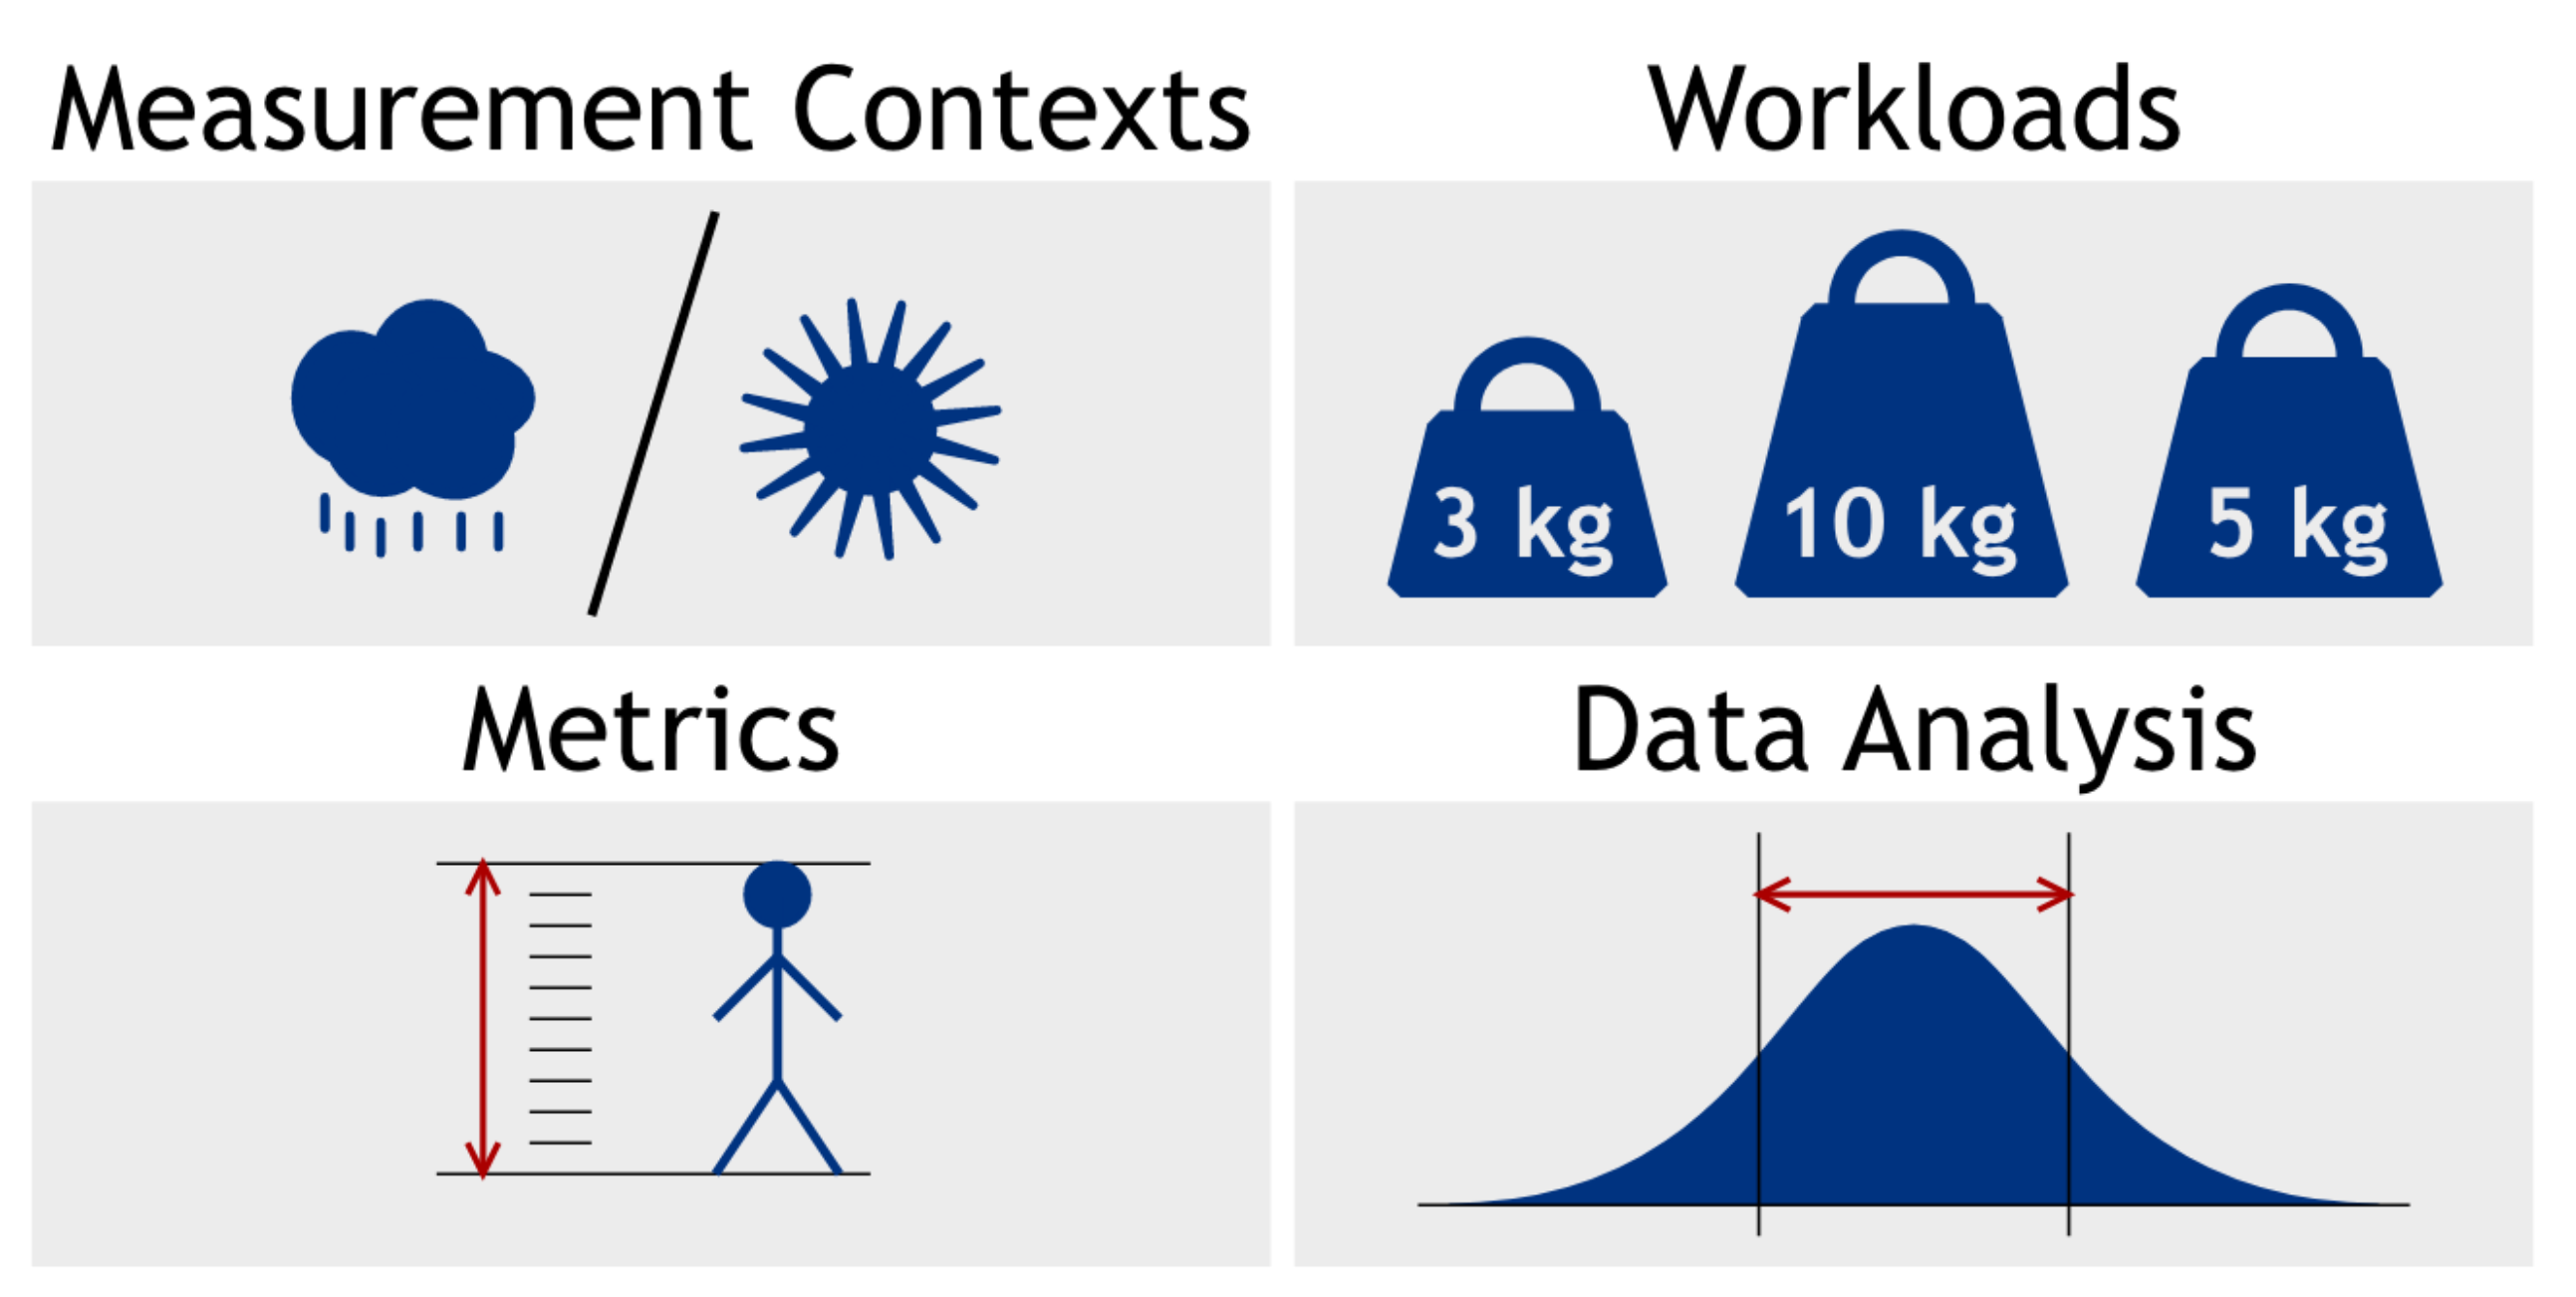
\includegraphics[scale=0.3]{imgs/componentsofanexperiment}}
    \caption{The proposed decomposition of an experiment~\cite{stephen_evaluate_2012}}\label{fig:soa_expermiment_component}
\end{figure}
Finally, to make unify the benchmarking methodology across different research works in the field of computer science, we can cite the paper~\cite{stephen_evaluate_2012}. In their approach they  divided any empirical experiment into four  components.
Figure \ref{fig:soa_expermiment_component} presents these components, which are:
\begin{enumerate}
    \item \emph{measurement contexts} that indicate the software and hardware components that will alter or remain constant during the experiment.
    \item \emph{workloads} which identify the benchmarks to use in the experiment, as well as their inputs;
    \item \emph{metrics} that specify the attributes to be measured and how to assess them.
    \item \emph{Data analysis} show how to examine data and evaluate the outcomes of the analysis to offer insight into the assertions that arise from the study.
\end{enumerate}

The work of this thesis will be based on this approach, since it provides a unified methodology for benchmarking and evaluating the performance of different systems.

% %%%%% move it to SOA maybe 
% \subsection{Virtual Machines}
% First option should be using \emph{Virtual Machines} (VM), which gives researchers the freedom to choose the most appropriate tools, software and operating system that they are the most comfortable with, without paying the price to change the actual working environment, which will give them eventually more control over the dependencies and the execution environment.
% Moreover, using a VM addresses the \emph{replication crisis} thanks to the virtual images, as even the most complex architecture can be reproduced easily by instantiating a copy of the image.
% Since the virtual machines are agnostic to the host architecture, researchers will not have to worry about where and how their experiments are replicated, because they have already setup the execution environment.
% Another advantage of VM is the snapshot mechanism, as it allows researchers to create backups and revert some changes with simple clicks. 
% Last but not least, thanks to the isolation, virtual machines push the reproducibility further by allowing the future usages to see all the variables---controlled and uncontrolled---and do other analysis without dealing with any dependencies.
% In his paper~\cite{howe_virtual_2012}, Bill Howe lists the benefits of using VM in researchers experiments, including the economical impact and cultural limitation to a such approach.
% In particular, VM allow them to have control over the resources, the dependencies, and the execution environment.
% Moreover, thanks to snapshots, deploying a software is easily achieved by instantiating a copy of that image.
% However, this choice comes with a certain cost.
% Because of the hypervisor, software will build on two kernels---the virtual machine (guest) one and the host machine one---which will provide a noticeable overhead, and will impact the performances of the system-under-test.
% Therefore, we cannot use VM for experiments that are related to performance.
% Another limitation of VM is the the isolation.
% While this feature prevents the experimental environment from any undesirable interference from the outside world, this interaction may be required---especially when the experiment is dependent to an external 
% As Stephen M. Blackburn~\emph{et~al.} cited in their paper "evaluate collaboratory"~\cite{stephen_evaluate_2012}, one of the major pitfalls of the measurement contexts is the inconsistency, which can be translated here by the fact that the production context is not the same as the benchmarking one.

% Another difficult part for practitioners is to generalize the claims they reached beyond the lab conditions.
% Are they appropriate?
% Are they consistent and are they reproducible?
% To answer those questions, the community agreed on some wellknown benchmarks to represent a specific concern of the production world.
% One can site as an example the Dacapo~\cite{DaCapo:paper} and Renaissance~\cite{renaissance} benchmark suites for Java applications, or the CLBG benchmark suite for comparing programming languages\footnote{\url{https://benchmarksgame-team.pages.debian.net/benchmarksgame/index.html}}.
% Although they do not cover all the cases, the community agrees on their relevance and representativeness.

% In addition to these benchmarks, a new category of testing techniques has emerged to simulate the worst cases of the production environments. This new category of benchmarking called performance tests\cite{pradeep2019pragmatic}, which are benchmarks meant to evaluate the behavior of software under stress situations. We can use the Gatling\footnote{\url{https://gatling.io/}} as an illustration for web applications stresser and stress-ng for hardware heavy workload perormance measurements~\cite{king2017stress}.

\section{Energy Measurement}\label{sec:soa_energymeasurement}
Now that we have discussed the importance of benchmarking and the different approaches that can be used to evaluate the performance of a system, we will focus on energy measurement, which will be the main metric in this thesis. Therefore, in this section, we will discuss the different approaches that can be used to measure the energy consumption of a system.
Many studies have been conducted to estimate such energy consumption. that varies from static analysis of the source code to infer its energy consumption like \citeauthor{pereira_helping_2017} where they provided a tool to highlight the most energy consuming parts of the code \cite{pereira_helping_2017}.
The key advantage of this approach is that it allows you to estimate a program's energy usage without actually executing it.
Unlike program complexity, energy consumption is strongly dependent on the execution environment.
As a result, static analysis may not accurately represent the behavior of the same program when run in a production context.
To address the issue of representativeness, many researchers measure the energy consumption of programs as they run. As a result, we will get more accurate results.
There are various tools for measuring energy, and they cover a wide range of applications depending on how accurate and precise the results must be on the one hand, and the price that practitioners are prepared to pay for such accuracy and precision on the other.

% depends on the scientific usage there are two apporaches :
% 1. extern one or independent : when the most of researchs are using
% the benifits of this is the simplicity of instalation however we pay the price either with a lack of temporal resolution ( low frequency ) or the spatial granularity
% ( most of them measure the energy consumption of the whole machine )
% 2. dedicated one , they are based on the instrumentation of some parts of the computer , however they have a high cost and they are defficult to scale since they require an instrumentation of the execusion environment.
According to \citeauthor{hackenberg2014hdeem} there are four main criterions to evaluate an energy measurement tool \cite{hackenberg2014hdeem}
\begin{itemize}
    \item \emph{Spatial granularity}: the more specific the target of monitoring we are able to measure, the more efficient we can do optimization since we will know what causes the pitfalls of the energy consumption.
    \item \emph{Temporal granularity}: same as spatial granularity, temporal granularity helps us to identify the sequence of code that need to be optimized.
    \item \emph{Scalability}: this is mainly related to the cost of the tools and the ease of their integration for our system.
    \item  \emph{Accuracy}: to eliminate extra hazards and get more representative measurement.
\end{itemize}

We believe that accuracy can be extracted from those criteria since it is a result of the combination of the two first ones. Therefore, we will focus more on the first 3 criteria later on. Below, we will discuss some of the well known tools that are used in literature.
\subsection{Hardware Tools}
Nowadays, most high-performance computing systems (HPC) implement a tool to report the energy consumption of the nodes for the sake of monitoring and administration.
Those tools are mainly integrated with the power supply units (PSU) or power distribution units (PDU).
Then, they provide an interface and a log to follow the history of the energy consumption.
despite their scalability and ease of integration.
Such tools lack both spatial and temporal granularity since they monitor the whole energy of the nodes and, most of the time, have a very low sampling frequency.
Most of those tools are provided directly by the manufacturers.
Such as \emph{IBM EnergyScale technology}~\cite{mccreary2007energyscale,caldeira2014ibm,caldeiraibm} or \emph{Dell poweredge}~\cite{lovicott2009thermal}, MEGware Cluststafe~\cite{breitbart2015case}.
As said earlier, the true purpose of those tools is more monitoring than analyzing the energy consumption.
%% add something to link with wattsup pro 
WattsUp Pro, is a device that can be installed between the power source of the machine and the system under test.
It allows a sampling frequency up to 1\,Hz and has a internal memory to store a wide variety of data, such as the maximum voltage, current, that later can be exported via USB port for personal usage or lined to some graph programs like Logger Pro or LabQuest.
The main advantage of this tool is the ability to monitor the energy consumption from a different device which will reduce the risk of interference with the energy consumption of the test % a revoir 
\cite{hirst2013watts}

Despite his high temporal granularity, wattsup pro lacks in term of spatial granularity since it monitors the energy consumption of the whole system.
To have a finer granularity we need to isolate the energy consumption of each component.
For this, we will need more intrusive tools such.

%% THIS IS FOR GPU %%% 
% GPU TESLA \cite{burtscher2014measuring}

% NVML\cite{fahad2019comparative}
%%%% 

PowerMon and its upgraded version powerMon2 \cite{bedard2010powermon} are based on an micro-controller chip that can monitor up to 6 channel (8 for powermon2), simultaneously.
Therefore, we are able to monitor the power consumption of 4 devices at the same time.
The frequency sample of this tool is up to 50\,Hz, with an accuracy of 1.2\%.
Powermore2 comes with smaller size that can fit within 3.5 inches rack drive.

PowerInsight~\cite{laros2013powerinsight} is another fine-grained measurement tool that is based on an ARM bagelbone processor~\cite{coley2012beaglebone}, which is able to measure up to 30 channel simultaneously with a frequency of 1KHz per channel.

% On the other hand, GreenMiner \cite{hindle2014greenminer}, %%i dont think that  mobile measurement will be relevent for my case 
powerpack~\cite{ge2009powerpack} in the other hand is an api that synchronizes the data gathered from other monitoring tools such as Watt’s Up Pro, NI and RadioShack pro and the lines of code. %% maybe remove this one from the list because it is not well known.

Other monitor tools have been realized by the manufactures, such as IBM Power executive~\cite{koomey2011growth}, which allows their customer to monitor the power consumption and thermal behavior of the of BladeCenter systems in the data center.


Accoring to the work of \citeauthor{vasques2019review} and\citeauthor{wang2018modelling}
The CPU is the part responsible for the most energy consumption in a data center\cite{vasques2019review,wang2018modelling}. Hence, the finer we go to measure this energy consumption, the better it is for our work.
Fortunately, Intel and later AMD proposed a tool that estimates the power consumption of different parts of the CPI based on counter performances.
RAPL (\emph{RUnning Average Power Limit}) \cite{hackenberg2013power,hackenberg2015energy} is a set of registers that was introduced by Intel in their CPU since Sandy bridge generation, and later it was followed by AMD, since Family 17h Zen.


\begin{figure}[!hbt]
    \centering{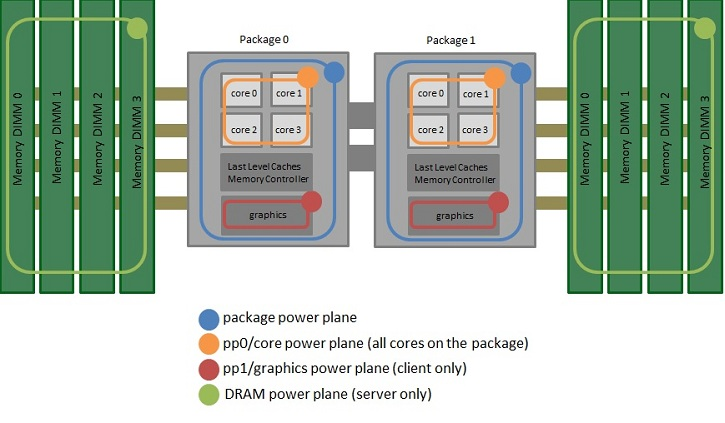
\includegraphics{imgs/power-planes-rapl}}
    \caption{INTEL RAPL scopes
    }\label{fig:rapl-domaine}
\end{figure}

Figre~\ref{fig:rapl-domaine} shows the different scopes  thhat can be monitored using RAPL.
The CPU package can be monitored for both server and desktop processors. However, DRAM is only available on server CPUs, whilst the integrated GPU is only available on desktop processors.
The advantage of such an approach is that the absence of any intrusive measurement tools.
Furthermore, they have a high temporal granularity with a sampling frequency up to 1\,KHz~\cite{ilsche_power_2015}.

With similar approach, we can find NVIDIA reporting tools, such as GPU TESLA \cite{burtscher2014measuring} and the NVML library~\cite{fahad2019comparative}.

\subsection{Software Tools}
Software-based measurement tools are based on other hardware tools to monitor energy use. Granularity is the core value of these technologies, unlike hardware tools, which only provide the total energy usage of the system/component (computer, server, motherboard, etc.) for most cases.
Because they are frequently constructed on empirical estimations and data learning methods, they drop in accuracy.

Many software measuring tools understand the behavior of a power model and provide estimates of energy usage.
This model is then used to allocate the observed energy consumption among different execution entities, such as processes, control groups, threads, or even code lines.

The first examples of software measurement tools are PowerAPI~\cite{colmant2018next}, SmartWatts formula~\cite{fieni2020smartwatts} and SelfWatts~\cite{fieni2021selfwatts}.
These tools collect global energy consumption measurements from RAPL and use other system events such as cache misses/hits and CPU frequency evolution (DVFS) via a sensor to construct a power model of the control groups (system control groups, docker containers, kubernetes pods, etc.) using a Ridge regression.
The model continuously learns and improves its precision of real-time energy usage data with a maximum frequency of 100 Hz.
The instrument has a decentralized, lightweight design.
Only the lightest sensors required for data collection and transmission are put into the monitored devices.
The SmartWatts formula is then executed on the primary server in order to construct the model that permits assigning the energy usage for each operating control group.
PowerAPI is only compatible with Linux on a bare-metal physical computer.
\\
WattWatcher~\cite{lebeane2015watt} is a multi-core power measuring framework that provides process-level energy measurements.
This program uses power models to predict process energy usage. It uses CPU events which are passed from the measured node to a model generator node in order to construct the power model. It works by combining a description of the CPU with a list of the hardware events through multiple calibration phases in order to build a robust model.

Joulemeter~\cite{kothari2009joulemeter,jagroep2017energy} is a Microsoft software that estimates the energy usage of Windows running applications down to the process level by using power models (for CPU, memory, and drives).
It employs low-overhead power models to infer power consumption from resource utilization during runtime, and it provides power limiting features for virtual machines.
Previous Joulemeter tests~\cite{jagroep2015profiling} demonstrated that the instrument provides a less accurate estimation of energy use that differs greatly from the real one.
To adjust its models to the hardware on which it operates, Joulemeter must first go through a calibration step.
It is able to only monitor one process at a time with a frequency of 1\,Hz.

JRAPL is another example of an energy measurement tool estimating tool that has been utilized in a variety of publications~\cite{guimaraes2016some,liu_data-oriented_2015}.
This software enables for the energy usage of Java programs, functions, or even a block of code lines to be profiled and measured.
The measurements are heavily reliant on the data supplied by RAPL.
As a result, the global energy consumption collected by RAPL between two timestamps (the start and finish of the code to measure) is used to calculate the energy consumption of the Java code.
Tests using jRAPL should be done on a well-configured machine to minimize the impact of the operating system and user operations on the overall energy consumption of jRAPL.

Another process-level energy usage measuring tool is Jolinar~\cite{islam2016measuring,noureddine2016jolinar}.
The tool does not need a calibration phase and relies on pre-established power models based on hardware metrics (TDP, disk I/O rate, and so on).
These settings must be identified and supplied by the user for his machine.
Jolinar is only capable of measuring the energy consumption of one application at a time.
At the end of the execution, the tool provides the CPU, DRAM, and disk energy usage of the main process.
Jalen~\cite{noureddine2015monitoring} is another tool that profiles and monitors the energy usage of a Java program.
Unlike jRAPL, Jalen is able to cover the scope down to the function level.It gathers data using code instrumentation and statistical sampling at a predetermined pace.
Because of the overhead that code instrumentation may incur, the authors recommend utilizing the second option.
Every 10 ms, Jalen records the JVM's stack trace together with the CPU time of threads and computes statistics about method calls.These statistics are then utilized to calculate each method's energy usage.

% selfwatts \cite{fieni2021selfwatts}
% powerjoular \cite{noureddine2022powerjoular}

% \subsection{Hybrid Tools}
% split hardware tools into extern and embeded tools 

% Simgrid simulation of power consumption of parallel aplication using simgrid \cite{heinrich2017predicting}

% impact of manifacturing process on the energy variation \cite{coles2014comparing}

% different energy consumption between identical processers [ idle and hight load ]\cite{von2016variations}

% the temperature is the main raison a high energy variation \cite{wang2018potential}

% external factors are impact on the energy variation \cite{mukherjee2009spatio}

% the place of the server in the room doesn't affect the energy variation \cite{diouri2013your}

% comparaison of three measuring tools and they did exhebit 10\% variation each time \cite{inadomi2015analyzing}

\section{Energy Variation}\label{sec:energy_variation}
In theory, using identical CPU, same memory configuration, similar storage and networking capabilities, should increase the accuracy of physical measurements.
Unfortunately, this is not possible when it comes to measuring the energy consumption of a system.
Applying the benchmarking guidelines and repeating the same experiment with in the same configuration are not sufficient to reproduce the the same energy measurements, not only between identical machines, but even within the same machine.
This difference---also called \emph{energy variation} (EV)---has become a serious threat to the accuracy of experimental evaluations.

Figure~\ref{fig:motivation} illustrates this variation problem as a violin plot of $20$ executions of the benchmark \emph{Conjugate Gradient} (\textsf{CG}) taken from the \emph{NAS Parallel Benchmarks} (NBP) suite~\cite{Bailey:1991:NPB:125826.125925}, on $4$ nodes of an homogeneous cluster (the cluster \textsf{Dahu} described in Table~\ref{table:g5k}) at 50\,\% workload.
We can observe a large variation of the energy consumption, not only among homogeneous nodes, but also at the scale of a single node, reaching up to $25\,\%$ in this example.

\begin{figure}%[!htb]
    \center{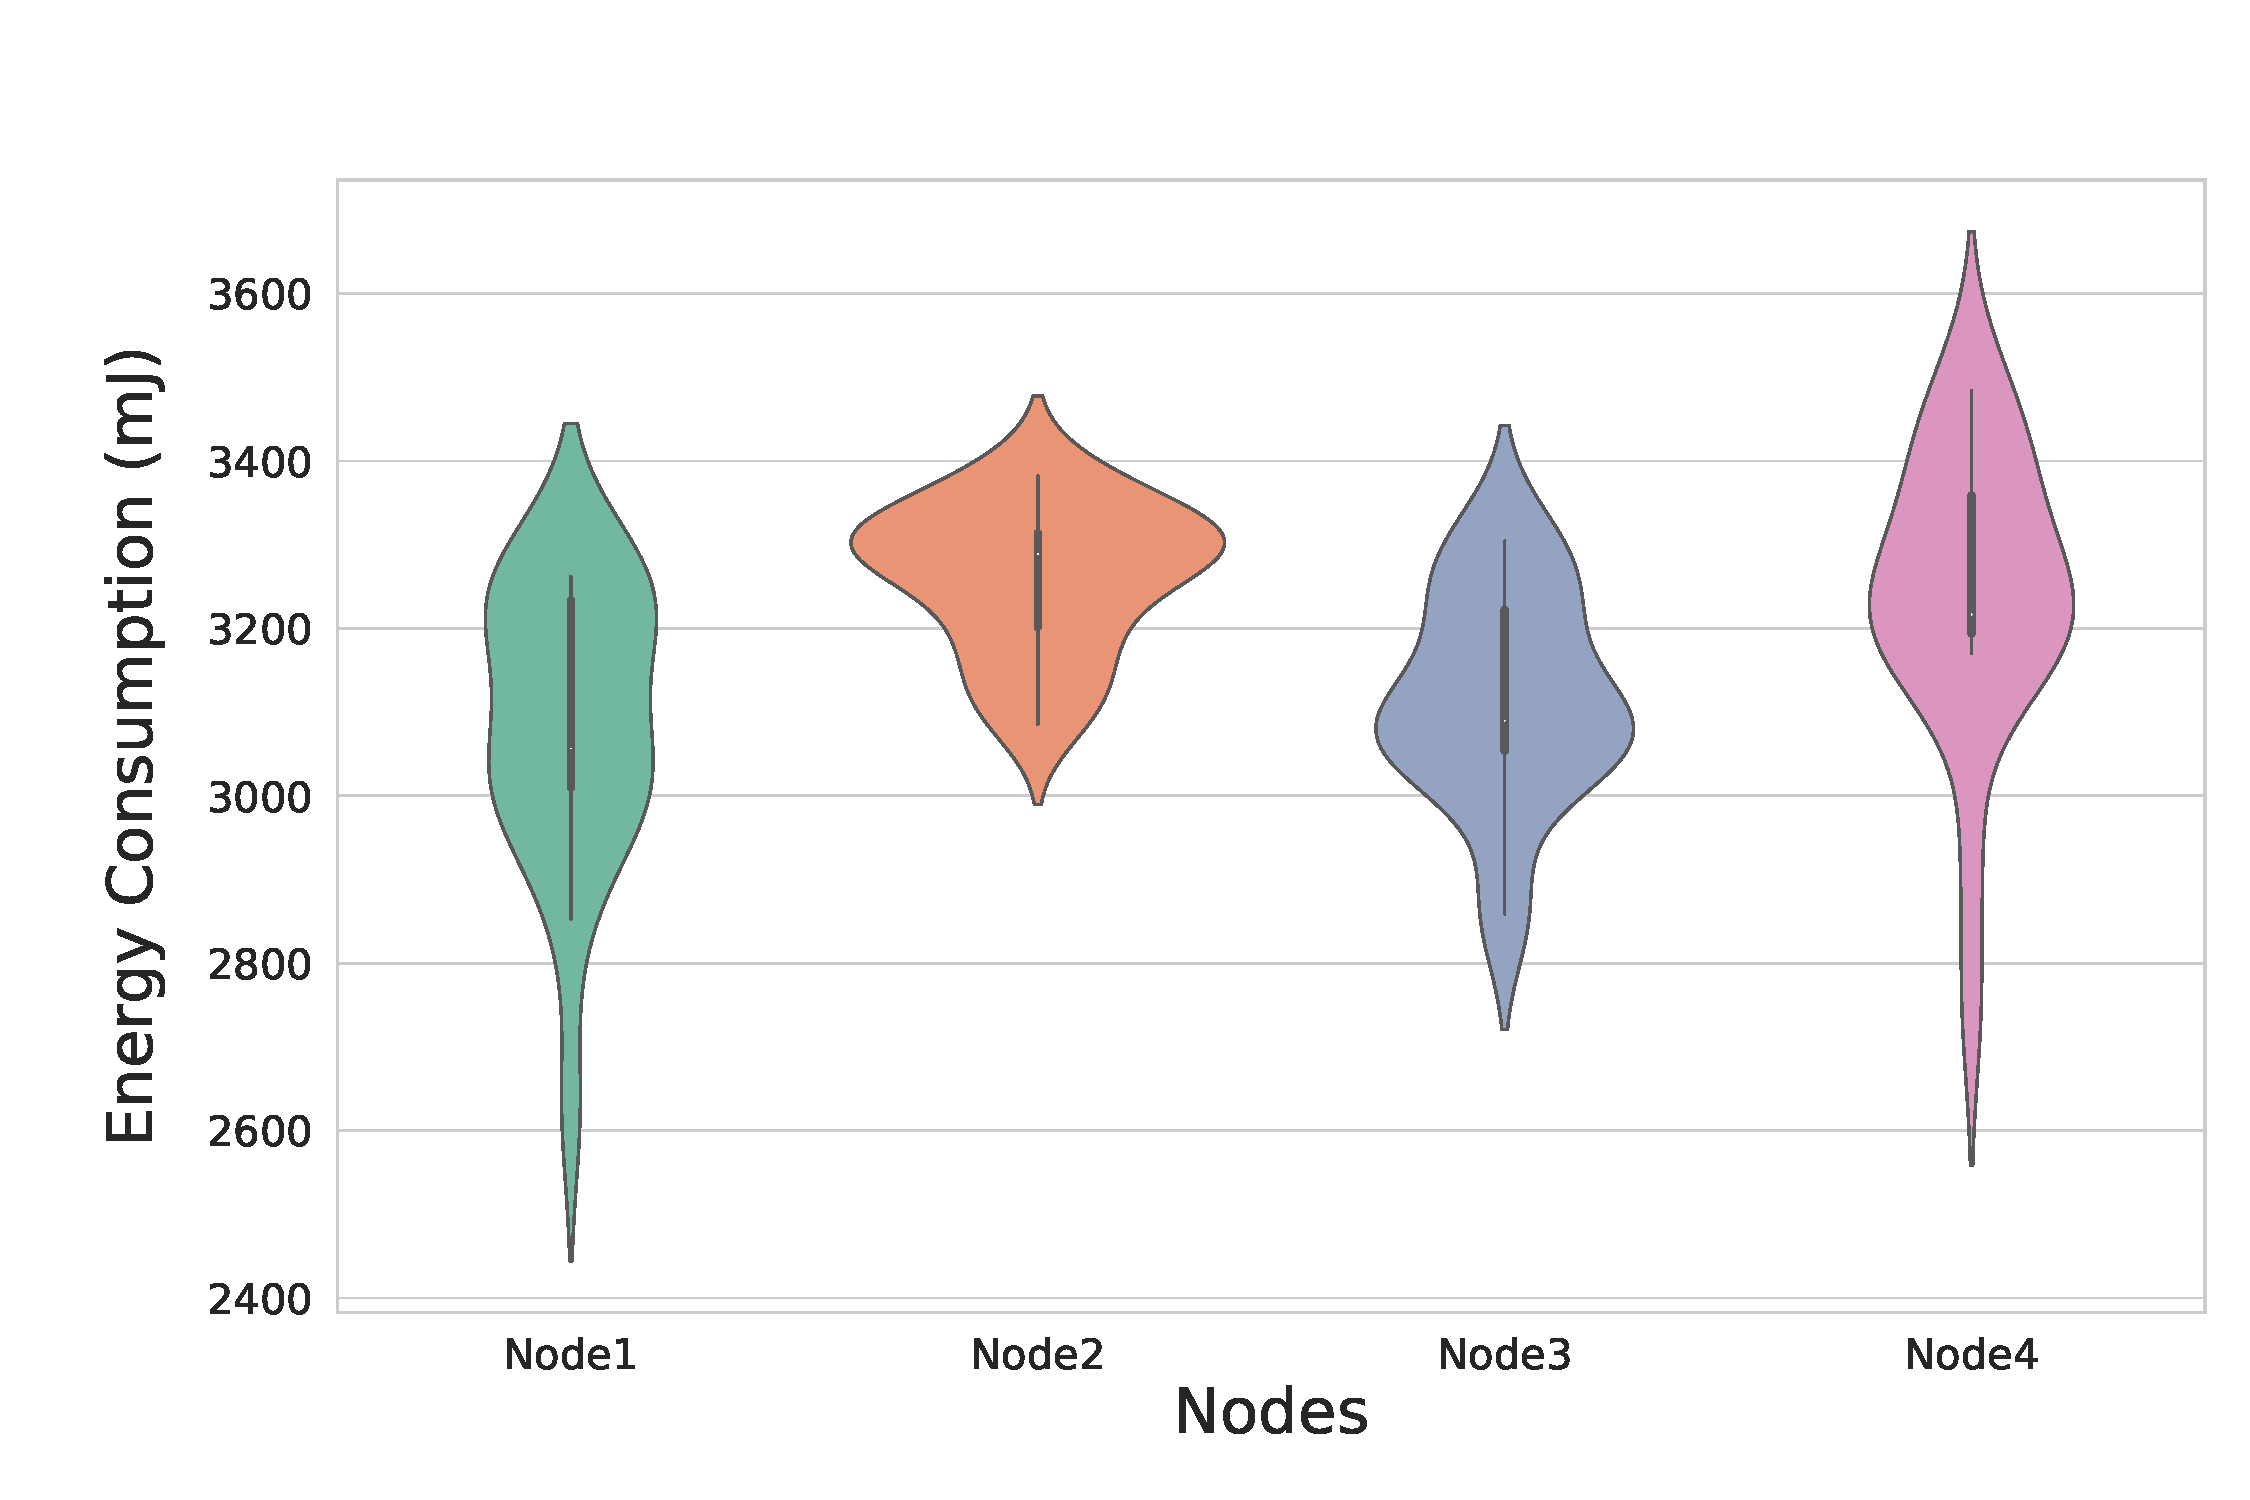
\includegraphics[width=.9\linewidth]{imgs/motivation}}
    \caption{CPU energy variation for the benchmark \textsf{CG}}\label{fig:motivation}
\end{figure}
%% state of the art 
Some researchers started investigating the hardware impact of the energy variation of power consumption.
As an example, one can cite~\cite{borkar_designing_2005,tschanz_adaptive_2002} who reported that the main cause of the variation of the power consumption between different machines is due to the \textbf{CMOS} manufacturing process of transistors in a chip.
\cite{heinrich_predicting} described this variation as a set of parameters, such as CPU Frequency and the thermal effect.
\subsection{Studying Hardware Factors}
This variation has often been related to the manufacturing process~\cite{coles_comparing_2014}, but has also been a subject of many studies, considering several aspects that could impact and vary the energy consumption across executions and on different chips.
On the one hand, the correlation between the processor temperature and the energy consumption was one of the most explored paths.
Kistowski~\emph{et~al.} showed in~\cite{joakim_v_kisroski_variations_2016} that identical processors can exhibit significant energy consumption variation with no close correlation with the processor temperature and performance.
On the other hand, the authors of~\cite{wang_potential_2018} claimed that the processor thermal effect is one of the most contributing factors to the energy variation, and the CPU temperature and the energy consumption variation are tightly coupled (up to 16\% increase in the variation when the temperature changed from 37.7°C to 74.5°C ).

This exposes the processor temperature as a delicate factor to consider while comparing energy consumption variations across a set of homogeneous processors.%, but also, if a same workload can cause the CPUs to reach different temperatures.

The ambient temperature was also discussed in many papers as a candidate factor for the energy variation of a processor.
In~\cite{ranka_energy_2009}, the authors claimed that energy consumption may vary due to fluctuations caused by the external environment.
These fluctuations may alter the processor temperature and its energy consumption.
However, the temperature inside a data center does not show major variations from one node to another.
In~\cite{el_mehdi_diouri_your_2013}, El~Mehdi~Dirouri~\emph{et~al.} showed that switching the spot of two servers does not affect their energy consumption.
Moreover, changing hardware components, such as the hard drive, the memory or even the power supply, does not affect the energy variation of a node, making it mainly related to the processor.
This result was recently assessed by~\cite{wang_potential_2018}, where the rack placement and power supply introduced a maximum of $2.8\,\%$ variation in the observed energy consumption.

Beyond hardware components, the accuracy of power meters has also been questioned.
\citeauthor{inadomi_analyzing_2015}~\cite{inadomi_analyzing_2015} used three different power measurement tools: RAPL, Power Insight\footnote{\url{https://www.itssolution.com/products/trellis-power-insight-application}} and BGQ EMON.
All of the three tools recorded the same $10\,\%$ of energy variation, that was supposedly related to the manufacturing process.

\subsection{Mitigating Energy Variations}
Acknowledging the energy variation problem on processors, some papers proposed contributions to reduce and mitigate this variation.
In~\cite{inadomi_analyzing_2015}, the authors introduced a variation-aware algorithm that improves application performance under a power constraint by determining module-level (individual processor and associated DRAM) power allocation, with up to $5.4\times$ speedup.
The authors of~\cite{hammouda_noise-tolerant_2015} proposed parallel algorithms that tolerate the variability and the non-uniformity by decoupling per process communication over the available CPU.
Acun~\emph{et~al.}~\cite{acun_variation_2016} found out a way to reduce the energy variation on Ivy~Bridge and Sandy~Bridge processors, by disabling the Turbo~Boost feature to stabilize the execution time over a set of processors.
They also proposed some guidelines to reduce this variation by replacing the old---slower---chips, by load balancing the workload on the CPU cores and leaving one core idle.
They claimed that the variation between the processor cores is insignificant.
In~\cite{chasapis_runtime-guided_2016}, the researchers showed how a parallel system can be used to deal with the energy variation by compensating the uneven effects of power capping.

In~\cite{marathe_empirical_2017_m}, the authors highlight the increase of energy variation across the latest Intel micro-architectures by a factor of $4$ from Sandy~Bridge to Broadwell, a $15\,\%$ of run-to-run variation within the same processor and the increase of the inter-cores variation from $2.5\,\%$ to $5\,\%$ due to hardware-enforced constraints, concluding with some recommendations for Broadwell usage, such as running one hyper-thread per core.
%  NOTE :/this might be interesting for greeFaaS

\section{Energy optimisation}\label{section:soa_energyoptimization}

We will now turn our focus to the energy optimisation challenge after considering the various ways for measuring energy consumption in computers and understanding the energy variation problem.
Over the previous decade, there has been a considerable increase of interest in this field, with many papers proposing different approaches to reduce the energy consumption of software applications. This section will passthrough the main contributions in this field, and will focus on the two following parts.

\subsection{Energy optimization in the conception phase}

The first part of this section will focus on energy optimisation in the conception phase, where the goal is to make the final product use less energy by choosing the best set of programming languages, tools, libraries, etc. It also includes all the work and optimizations that developers can do to the source code to make the software use less energy when it is running.

We start with the work of \citeauthor{pereira_energy_2017} \cite{pereira_energy_2017} where they  did an energy consumption comparison analysis of the most popular programming languages.
Using the Pareto optimum~\cite{hochman1969pareto}, the paper  provides recommendations on how to combine some of these languages to enhance code quality while taking into account execution time, memory utilization, and energy consumption. Some of the study's findings demonstrate that interpreted languages, such as Python, have lower energy efficiency than compiled languages, such as C or Rust. The research also offers language combinations that developers might use together to improve energy economy, execution speed, and memory utilization.
This paper's findings were based on the game benchmark, which is the most famous set of benchmarks that compares several programming languages.


\citeauthor{couto2017towards} ~\cite{couto2017towards}investigated the influence of programming language choice on the energy consumption of software during execution. In their paper~\cite{couto2017towards}, they examined a set of computing problems written in ten well-known programming languages while observing the energy required when running each language. They also found that there are interesting situations in which slower languages use less energy than faster ones, even though fast languages are usually the ones that use the least energy.
Finally, they produced an energy efficiency rating of programming languages.
The paper~\cite{bujnowski2020java} compared the energy, performance and database response time of web applications written in Java versus those written in Kotlin. They discovered that there is no statistically significant difference in CPU load between individual measurements( less than 2\%) 2. Howerver, Kotlin implementation has never earned the best results in any collection of measurements.

Other works that have studied the impact of the website technology on the energy conusmptuon,\cite{philippot_characterization_2014,manotas_investigating_2013}. In their work~\cite{philippot_characterization_2014},\citeauthor{philippot_characterization_2014} measured the computer resources used during the loading of a website in a browser, such as memory utilization and energy consumption, for over 500 websites and proposed some best practices for developers.

Other works examined software energy consumption efficiency through source code changes and optimizations. For example, some papers [42, 122] studied the effect of Java collections on energy consumption, depending on the collection size and/or the most executed tasks on the collection (insertion, removal, search). They provided some insights into the energy efficiency of some collections for multiple scenarios. For example, Hasan et al. [52] compared the energy consumption of several Java data structures, analyzing the bytecode using the Wala framework8 and assessing the evolution of the energy consumption in different scenarios (insertion at the beginning, iteration, etc.). They also used some automated replacement of LinkedList and ArrayList to simulate best-and worst-case energy consumption scenarios in real production applications. Their study showed that using inappropriate collection can cause up to 300\% of energy consumption inefficiency.

As for the impact of the source code on the energy consumption, we can cite~\cite{pinto_comprehensive_2016,fernandes_assisting_2017} where the authors investigated the impact of Java collections on energy usage based on collection size and its usage (insertion, removal, search) and They provide some insights into the energy efficiency of specific collections under various scenarios.

\citeauthor{hasan_energy_2016}~\cite{hasan_energy_2016} examinind the energy consumption of multiple Java data structures, analyzing the bytecode and evaluating the change in energy consumption in various circumstances(research,insertion, deletion, etc.). They also simulated best- and worst-case energy usage scenarios in real-world production systems by replacing the LinkedList and ArrayList, and discovered that incorrect collection can result in a 300\% increase in energy consumption.

Other studies\cite{longo_reducing_2019,kumar_energy_2017} looked into the energy use of Java primitive types, string operations, and the use of exceptions, loops, and arrays. \citeauthor{kumar_energy_2017}, for example, examined the energy usage of code snippets and micro-benchmarks and provided several conclusions, such as string concatenation would use less energy than StringBuilder and StringBuffer and static variables tends to consume 60\% more energy than instance variables.

\citeauthor{pereira_helping_2017} \cite{pereira_helping_2017} presented SPELL, a tool that helps developers spot energy leaks in their source code. Using a statistical spectrum-based analysis and JRAPL\cite{guimaraes2016some,liu_data-oriented_2015}, the tool locates energy-inefficient code fragments. According to the authors, it is language and context independent.

\subsection{Energy optimization in the execution phase}

The second part of this section will focus on energy optimization in the execution phase, where the goal is to optimize this energy consumption for already developed software without making changes to the source code.The goal is to set up and create an environment in which software can run with the least amount of energy. This could involve process scheduling, system tunning and so on.

We begin with Aequitas~\cite{ribic2016aequitas}, a system that allows parallel applications to live on power domains that are co-managed (sharing the same CPU). The technology is founded on the premise that coexisting programs can regard power-management hardware as a shared resource and collaborate on power management decisions. As a result, it accomplishes its purpose by scheduling these applications with a time slicing technique ( as anexamample round robin). The authors claim that their strategy achieves a 12.9\% improvement while incurring only a 2.5\% performance cost.

As for virtual machines, \citeauthor{kurpicz2016much}~\cite{kurpicz2016much}. analyzed the total energy consumption of a VM in a data center while emphasizing the static cost versus the dynamic one. In this paper , the authros introduced the transparent, reproducible, and predictive cost calculator model EPAVE for VM-based environments. The purpose of EPAVE is to provide the static cost of each VM on the server, which includes the air conditioning, power distribution, and the dynamic cost that is related to the VM activities.

The energy usage of virtual machine allocation and task placement has also been investigated~\cite{mishra_energy_2018}. In this article, The authors propose a method for mapping workloads to virtual machines and virtual machines to the physical ones (PMs) in an energy-efficient manner. To solve the problem of high heterogeneity of activities and resources, the jobs are categorised based on their resource requirements, and then the relevant VM is found, followed by the appropriate PM where the selected VM can be deployed Using a cloud simulator, the authors claimed The suggested technique saves energy by reducing the number of active PMs while also minimizing the makespan and task rejection rate.

Besides the impact of the orchestration of virtual machine, some works have been targeting the runtime of specific programming languages.Using the TPC-DS benchmark  , \citeauthor{chiba2018towards}~\cite{chiba2018towards} investigated the influence of HOTSPOT \footnote{\url{https://openjdk.org/groups/hotspot}} and J9\footnote{\url{https://www.eclipse.org/openj9}} on the performance of SQL-on-Hadoop systems (SPARK and TEZ) to reveal a three-fold disadvantage that one JVM can have over the other.
\citeauthor{oi_power_2011}~\cite{oi_power_2011} also compared the performance of HOTSPOT and J9. They demonstrated in their research that the relative performance of a JVM is affected by the workload. They discovered that HOTSPOT's performance ranged from 44\% to 289\% of J9, while its dynamic power consumption ranged from 2.7W to 7.2W, using the SPECjvm2008~\cite{shiv2009specjvm2008} benchmarks.

As for Python, \citeauthor{redondo_comprehensive_2015}~\cite{redondo_comprehensive_2015}compared the performance and memory usage of various Python implementations (CPython, Jython, IronPython, PyPy, and so on) using a 215 set of benchmarks to discover that Python2 performed better with short applications, while Python3 versions covered more tests due to compatibility and the fact that Python2 became obsolete.



% java vs python \cite{destefanis_statistical_2016}


% constant overheat of the jvm \cite{lafond2006energy}


% java collection energy footprint

% % java classes energy footprint \cite{hasan2016energy}

% framework to reduce java collections \cite{manotas2014seeds}

% energy consumption of java dev tools \cite{baskar2013experimental}

% Microbenchmarks on jvm \cite{longo2019reducing} \cite{baskar2013experimental}

% android automatic refactoring to reduce energy consumption \cite{banerjee2016automated} \cite{rodriguez2017reducing}

% java vs native c in android \cite{corral2014method}




% carbon footprint of training neural network \cite{strubell2019energy}

% SPELL, the energy leaks detector tool \cite{pereira2017helping}

% impact of energy profiling on software \cite{jagroep2017energy}

% impact of maintainability on software energy evolution \cite{calero2021does}

% definition \cite{wang1993grpc}

% comparison \cite{chamas2017comparing}

% empirical study \cite{de2021empirical}

% impact of website implementation on energy consumption \cite{philippot_characterization_2014} \cite{manotas2013investigating}

% PHP \cite{benmoussa_new_2019} \cite{das_comparison_2016}

% simulation of web cache \cite{cardenas_performance_2005}

% java spring analysis \cite{gajewski_analysis_2019}

% performance \cite{mishra2021web}


% cross compiler benchmarking \cite{yet2016cross}

% \subsection{Python}

% web frameworks on python \cite{pankiv_concurrent_nodate}

% hope library \cite{akeret_hope_2015}

% bytecode effect \cite{ben_asher_effect_2009}

% numba \cite{crist_dask_2016}

% intel python \cite{li_boosting_2016}

% python 2 vs 3 \cite{modzelewski_pyston_2020}

% python runtime performances \cite{redondo_comprehensive_2015} \cite{murri_performance_2013}

% static vs dynamic languages \cite{pang_what_nodate}

% concurent benchmark framework \cite{pankiv2019concurrent}


% \subsection{JVM}







% \subsection{benchmarking}
% %%%%%%%%%%% further references 
% NAS \cite{bailey_nas_nodate}
% statistics \cite{he_statistics-based_2019}
% benchmark crimes \cite{van_der_kouwe_benchmarking_2018}
% microservices \cite{grambow_benchmarking_2020}
% impact of webservers on web applications energy \cite{manotas_investigating_2013}
%%%%%%%%%%%%%%%%%  virtualisation 

%%%%%%%%%%%%% energy mitigation
%%****** mitigating the energy variation ******
% low-cost scalable variation-aware algorithm \cite{inadomi2015analyzing}

% reducing the energy variation by disabling turbo boost \cite{acun2016variation}

% reducing the energy consumption in parallel systems \cite{chasapis2016runtime}

% \cite{marathe2017empirical}



\section{Conclusion}
As we have seen in the state of the art, many methods have been proposed to reduce the energy footprint of the the ICT, which they can be applied in different parts of the lifecycle of the program, from consumption to the execution.
Furthermore, the execution phase took attention of many researchers because it is the part where the most energy is consumed.
This thesis will focus on that aspect as well.
However, unlike the most work that have been done on the hardware aspect, we will target the software impact on this energy, starting from the choice of the programming language up to how to tune some features of a frameworks in order to make the software consumes less energy.
To do so we use the empirical approach due to its consistency for the moment.
Unlike the performance, which is essentially related to the complexity of the algorithm, the energy consumption is more impacted by the hardware.
Therefore, to optimize the energy consumption we choose a spiral method based on 3 phases:
\begin{enumerate}
    \item execute the code,
    \item measure the program,
    \item infer the guidelines.
\end{enumerate}

\begin{figure}[!hbt]
    \center{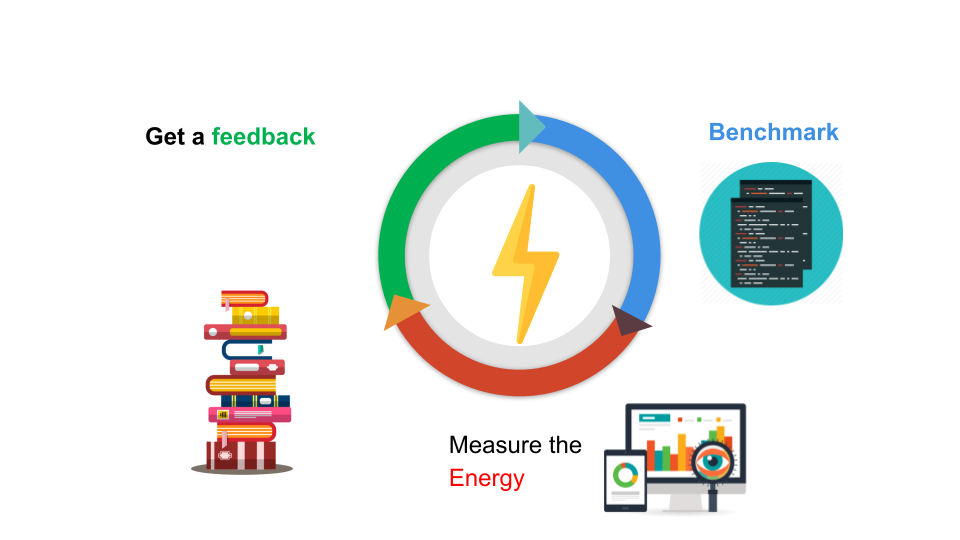
\includegraphics[scale=0.3]{imgs/greenbenchmarkcycle}}
    \caption{the spiral method of energy optimization }\label{fig:spirals}
\end{figure}

The aim of this work is to present a set of guidelines to create a benchmarking system to to measure the energy consumption of different programs.
After that, we will use this system to compare the energy consumption of different programming languages. We will extend the work of \citeauthor{pereira_energy_2017} to a closer distance to production environment by comparing a set of use cases.
Starting by GRPC framework, and a set of Web Frameworks.
Finally, we will discuss the impact of the execution environment on the energy consumption of two of the most famous programming languages Java and Python and present how can tunning the Virtual Machine can reduce the energy consumption.
